\documentclass[tikz,border=10pt]{standalone}
\begin{document}
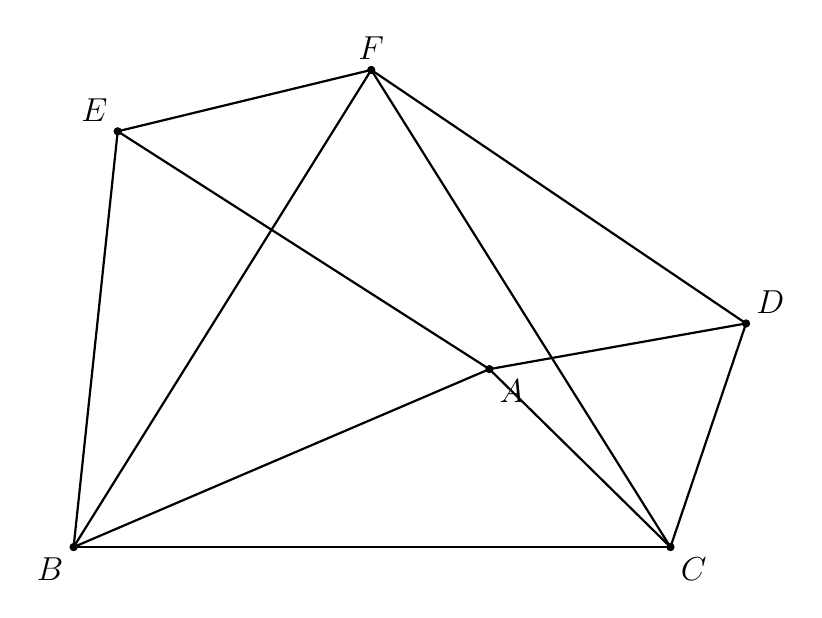
\begin{tikzpicture}[scale=1, line width=0.8pt, every node/.style={font=\large}]
  \coordinate (E) at (1.66,5.28);
  \coordinate (F) at (4.88,6.06);
  \coordinate (D) at (9.64,2.84);
  \coordinate (A) at (6.38,2.26);
  \coordinate (B) at (1.10,0);
  \coordinate (C) at (8.68,0);

  \draw (E) -- (F);
  \draw (F) -- (D);
  \draw (D) -- (C);
  \draw (C) -- (B);
  \draw (B) -- (E);
  \draw (B) -- (F);
  \draw (F) -- (C);
  \draw (E) -- (A);
  \draw (A) -- (C);
  \draw (B) -- (A);
  \draw (A) -- (D);

  \fill (E) circle (1.5pt);
  \fill (F) circle (1.5pt);
  \fill (D) circle (1.5pt);
  \fill (A) circle (1.5pt);
  \fill (B) circle (1.5pt);
  \fill (C) circle (1.5pt);

  \node[above left] at (E) {$E$};
  \node[above] at (F) {$F$};
  \node[above right] at (D) {$D$};
  \node[below right] at (A) {$A$};
  \node[below left] at (B) {$B$};
  \node[below right] at (C) {$C$};
\end{tikzpicture}
\end{document}
